\documentclass[a4paper]{article}

%maximum figure number
\setcounter{totalnumber}{5}

%plus minus
\newcommand{\mypm}{\mathbin{\smash{%
\raisebox{0.35ex}{%
            $\underset{\raisebox{0.5ex}{$\smash -$}}{\smash+}$%
            }%
        }%
    }%
}


%figure inside text
\usepackage{wrapfig}

%layout config
\usepackage{calc}
\setlength\textwidth{7in}
\setlength\textheight{10in}
\setlength\oddsidemargin{(\paperwidth-\textwidth)/2 - 1in}
\setlength\topmargin{(\paperheight-\textheight
-\headheight-\headsep-\footskip)/2 - 1in}

%sinuit
\usepackage{siunitx}
%image insertion
\usepackage{graphicx} %image settings
\DeclareGraphicsExtensions{.pdf,.png,.jpg}

%math
\usepackage{amsmath} %math
%\usepackage{cmbright} %math font

%font
\usepackage{kotex}
\usepackage{fontspec}
\ifx가가
\setmainhangulfont[Ligatures=TeX,
BoldFont={KoPubBatang Medium}]{KoPubBatang Light}
\setsanshangulfont[Ligatures=TeX,
BoldFont={KoPubDotum Medium}]{KoPubDotum Light}
\setmainhanjafont[Ligatures=TeX,
BoldFont={KoPubBatang Medium}]{KoPubBatang Light}
\setsanshanjafont[Ligatures=TeX,
BoldFont={KoPubDotum Medium}]{KoPubDotum Light}
\xetexkofontregime[puncts=prevfont, colons=prevfont, cjksymbols=hangul]{latin}
\fi

%줄간격
\usepackage{setspace}
%\usepackage{indentfirst}
\setstretch{1.2}
\everydisplay{\setstretch{1.2}}

%subfigure
\usepackage{subfigure}

\pagestyle{plain}
\title{물리 실험보고서 1}
\author{이한빈, 의예과 2016-13347}

\begin{document}


\numberwithin{equation}{section}
\maketitle

\section{Introduction}
	자연계에서 자기장이 발생하는 원인의 대부분은 운동하는 전하에 의한 전류이다.
	미소 전류 요소에 의해 발생하는 미소 자기장을 기술하는 법칙을 비오-사바르 법칙이라고 하며 다음과 같이 주어진다.
	\begin{equation}
		d\vec{B} = \frac{\mu_{0}}{4\pi} \frac{id\vec{s} \times \hat{r}}{r^2}
		\label{eq:biot}
	\end{equation}

	여기서 $d\vec{B}$은 미소 자기장, $d\vec{s}$는 방향은 전류의 방향과 같고 크기는 미소 전류요소와 길이와 같다.
	$r$은 $d\vec{s}$에서 해당자기장이 작용하는 위치까지의 거리이고 $\hat{r} = \frac{\vec{r}}{|\vec{r}|}$이다.
	따라서 전류가 흐르는 어떤 물체가 만들어내는 자기장을 구하고 싶다면 비오-사바르를 법칙을 적용한 후에 적분을 하면 된다. 
	\begin{figure}[h]
		\centering
		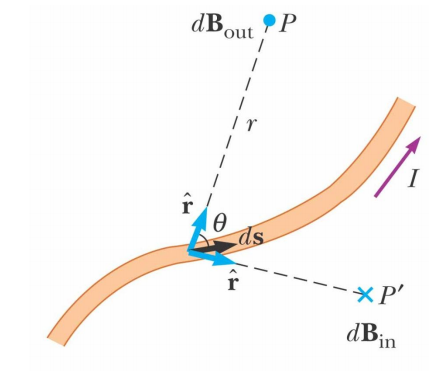
\includegraphics[width=0.3\textwidth]{img/biot.png}
		\label{fig:biot} 
		\caption{Biot-Savart Law}
	\end{figure}

\section{Method}
	준비물: 사각코일 1개, 파워 서플라이 1개, 솔레노이드 1개, 자석 1개, 나침반 1개, 홀센서, 홀-센서 전원장치, 컴퓨터, 방사형 평면, $30\si{cm}$ 자
	\subsection{홀센서 보정}
		홀센서는 자기장의 절댓값을 측정하는 것이 아니라 상대적인 값을 측정한다.
		홀센서로 자기장의 정확한 값을 얻기 위해서는 홀센서에 측정되는 자기장의 초깃값과 비례상수를 보정해주어야 한다. \\
		초깂값 보정: 자기장 발생장치의 전원을 모두 끄고 자기장이 발생할 수 있는 장치들로부터 홀센서를 최대한 멀리 떨어트린 이후에 그 때의 값을 0으로 설정한다. \\
		비례상수 보정: 규격을 알고 있는 솔레노이드를 이용하여 $20\si{mT}$의 자기장을 발생시킨 후 홀센서를 솔레노이드 중간에 넣고 이 때의 값을 $20\si{mT}$로 설정한다.
		*솔레노이드의 길이: $152\si{mm}$, 감은수: 500

	\subsection{전류에 따른 솔레노이드 자기장 변화 측정}
		솔레노이드의 전류를 $0.05\si{A}$씩 증가시켜가며 홀센서를 통해 솔레노이드 중앙에서의 자기장 세기를 측정했다.
		사용된 전류의 세기는 표(\ref{tab:soli})와 같다.
		\begin{figure}[h]
			\centering
			\begin{tabular}{c|cccccccc}
				\hline \hline
				전류(A) & 0.05 & 0.10 & 0.15 & 0.20 & 0.25 & 0.30 & 0.35 & 0.40 \\
				\hline \hline 
			\end{tabular}
			\caption{솔레노이드에 인가된 전류}
			\label{tab:soli}
		\end{figure} 

	\subsection{위치에 따른 솔레노이드 자기장 변화 측정}
		솔레노이드에 흐르는 전류를 $0.2\si{A}$로 고정한 후 솔레노이드 끝에서부터의 거리를 $1.5\si{cm}$단위로 줄여가며 자기장을 측정했다.
		측정에 사용된 끝에서부터의 거리는 아래 표(\ref{tab:sold})와 같다.
		\begin{figure}[h]
			\centering
			\begin{tabular}{c|cccccc}
				\hline \hline
				거리(\si{cm}) & 8.5 & 7.0 & 5.5 & 4.0 & 2.5 & 1.0 \\
				\hline \hline
			\end{tabular}
			\caption{솔레노이드 끝에서부터의 거리}
			\label{tab:sold}
		\end{figure}

	\subsection{방사형 평면 위에서의 자기장 측정}
		직선도선에 전류(0.43\si{A})를 흘려서 방사형 자기장을 만든 다음 중심거리와 각도를 바꾸어가며 자기장을 측정했다. \\
		중심거리 r은 $2\si{cm}$, $3\si{cm}$, $4\si{cm}$에서 각도 \ang{0}, \ang{30}, \ang{60}, \ang{90}로 하여 실험했다.

	\subsection{사각 코일 중심 축에서 중심으로부터의 거리에 따른 자기장 변화 측정}
		홀센서를 수평바닥으로 눕혀서 사각코일의 중심축 상에 위치시키고 그 때 프로그램에 나타는 $z$축 방향 자기장 크기를 측정했다.
		사각코일에 흐르는 전류는 0.42\si{A}였으며 전류는 장치를 전면에서 보았을 때 시계방향으로 흘렸다.
		실험에 이용한 거리는 표(\ref{tab:sagak})와 같다.
		\begin{figure}[h]
			\centering
			\begin{tabular}{c|ccccc}
				\hline \hline
				거리(\si{cm}) & 0 & 2 & 4 & 6 & 8 \\
				\hline \hline
			\end{tabular}
			\caption{사각코일 중심으로부터의 거리}
			\label{tab:sagak}
		\end{figure}

\section{Result}
	\subsection{홀센서 보정}
		측정된 솔레노이드의 길이는 152\si{mm}였으며 감은 수는 500이었다.
		솔레노이드를 무한히 긴 이상적인 솔레노이드라고 가정하면 중심에서의 자기장은 $B = mu_{0} n I$로 주어진다.
		따라서 20\si{T}의 자기장을 얻기 위해서 파워 서플라이에 인가해야할 전류는 $I = \frac{B}{\mu_{0} n} = \frac{20 \times 10^{-3}}{4\pi \times 10^{-7} \times 500 \div (152 \times 10^{-3})} = 0.43\si{A}$ 였다.

	\subsection{전류에 따른 솔레노이드 자기장 변화 측정}
		Method에서 인가한 전류에 따른 자기장은 다음과 같다.
		\begin{figure}[h]
			\centering
			\begin{tabular}{c|cccccccc}
				\hline \hline
				전류(\si{A}) & 0.05 & 0.10 & 0.15 & 0.20 & 0.25 & 0.30 & 0.35 & 0.40 \\
				\hline
				자기장(\si{mT}) & -2.85 & -5.95 & -8.88 & -11.65 & -14.34 & -16.54 & -18.17 & -19.27 \\
				\hline \hline 
			\end{tabular}
			\caption{솔레노이드에 인가된 전류에 따른 자기장}
			\label{tab:solire}
		\end{figure}

	\subsection{위치에 따른 솔레노이드 자기장 변화 측정}
		Method에서 인가한 솔레노이드 한 쪽 끝으로부터의 거리에 따른 솔레노이드의 자기장은 다음과 같다.
		\begin{figure}[h]
			\centering
			\begin{tabular}{c|cccccc}
				\hline \hline
				거리(\si{cm}) & 8.5 & 7.0 & 5.5 & 4.0 & 2.5 & 1.0 \\
				\hline
				자기장(\si{mT}) & 11.90 & 11.81 & 11.49 & 10.84 & 8.56 & 4.52 \\
				\hline \hline
			\end{tabular}
			\caption{솔레노이드 끝에서부터의 거리에 따른 자기장}
			\label{tab:soldre}
		\end{figure}

	\subsection{방사형 평면 위에서의 자기장 측정}

	\subsection{사각 코일 중심 축에서 중심으로부터의 거리에 따른 자기장 변화 측정}
	사각 코일 중심 축을 따라 중심으로부터의 거리를 바꿔가며 측정한 자기장의 변화는 다음과 같다.
	\begin{figure}[h]
			\centering
			\begin{tabular}{c|ccccc}
				\hline \hline
				거리(\si{cm}) & 0 & 2 & 4 & 6 & 8 \\
				\hline
				자기장(\si{mT}) & -3.23 & -3.07 & -2.83 & -2.44 & -2.24 \\
				\hline \hline
			\end{tabular}
			\caption{사각코일 중심으로부터의 거리에 따른 자기장}
			\label{tab:sagakre}
	\end{figure}

\section{Conclusion}
	

	

\section{Reference 및 부록}
	1. Halliday, D., Resnick, R., \& Walker, J. (2014). {\it{}Principles of Physics} (10th ed., Vol. 2). Hoboken, NJ: Wiley.
	\\ 

\end{document} 

%실험에서 개선할 점 등 피피티에서 봤던 거 모두 적어서 처리합시다